\chapter{Programmbeschreibung}
\label{chap:Programmbeschreibung}

\section{Packages}

Das Gesamte Programm ist in 4 Packages aufgeteilt. Es gibt ein Package model in dem die Datenstrukturen definiert sind.
Außerdem gibt es jeweils für die Eingabe, den Algorithmus und die Ausgabe ein eigenes Package.
Diese Packages sind untereinander unabhänging und loose über die im model Package definierten Datenstrukturen gekoppelt.
Außerdem gibt es natürlich das main Package das in der main() Methode alles verbindet.

\begin{figure}[h]
    \centering
    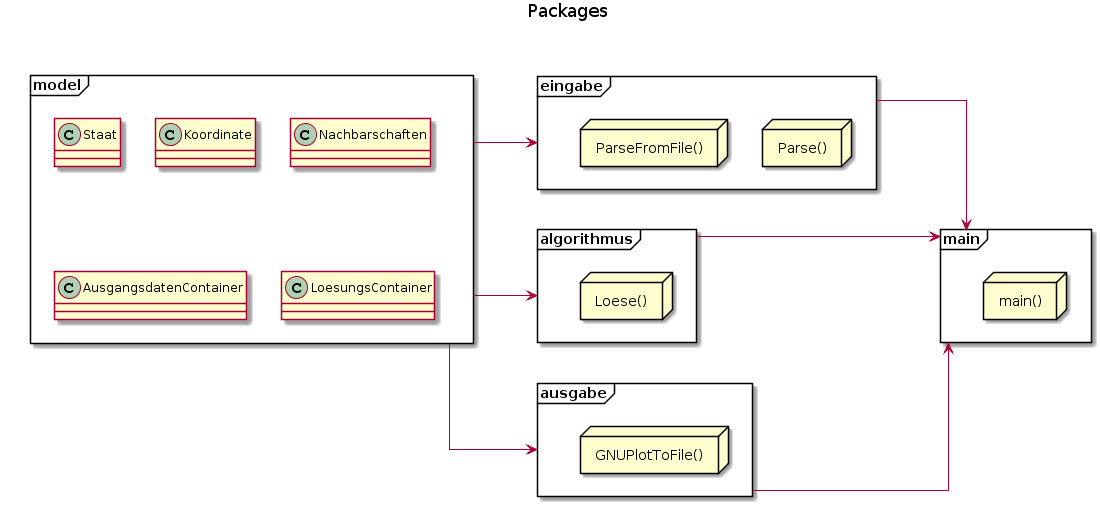
\includegraphics[width=0.9\textwidth,]{packages.png}
    \caption[]{Übersicht Packages}
\end{figure}

\subsection{Model}

Das Package Model enthält alle benötigten Klassen. Es wurde versucht die Klassenhirarchien möglichst simpel zu gestalten.

\begin{figure}[ht]
    \centering
    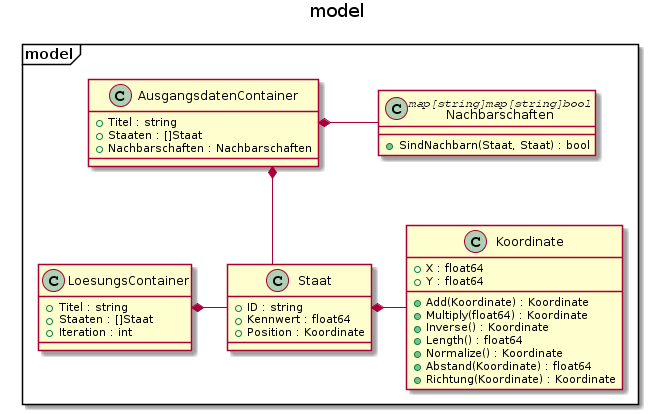
\includegraphics[width=0.9\textwidth,]{model.png}
    \caption[]{Package model}
\end{figure}

\subsubsection{Koordinate}

Die Klasse Koordinate beschreibt einen Vektor im $ R^2 $.
Sie besitzt eine  Reihe von Helfermethoden, die einfache Operationen wie die Streckung oder Addition von Koordinaten abbilden.

Als Datentyp für die Felder wurde float64 gewählt um eine möglichst große Genauigkeit zu haben.
Außerdem entahlten einige Methoden NaN Checks nach den Operationen und liefern im Zweifel einen Nullvektor zurück um numerische Instabilitäten zu vermeiden.

\subsubsection{Staat}

Die Klasse Staat ist die Datenstruktur für einen Staat und besteht aus einer string als ID, einem float64 als Kennwert und einer Koordinate als Position.


\subsubsection{Nachbarschaften}

Die Klasse Nachbarschaften beschreibt die Nachbarschaften zwischen den Staaten.
Sie ist ein typedef auf den Type map[string]map[string]bool, und beschreibt somit eine 2-dimensionale boolsche Set mit string Keys.
Durch das Ausnutzen von go's zero value erlaubt uns dies sehr einfache Prüfungen von Nachbarschaftsbeziehungen.
Mehr Informationen dazu lassen sich \href{https://blog.golang.org/go-maps-in-action}{hier} finden.
Die Methode SindNachbarn(Staat, Staat) prüft ob zwei Staaten Nachbarn sind. Dies ist dank der Verwendung einer Map in $ O(1) $ möglich.

\subsubsection{AusgangsdatenContainer}

Die Klasse AusgangsdatenContainer fasst alle zur Lösung des Problems notwendigen Informationen zusammen.
Sie dient als Schnittstellendatentyp zwischen Eingabe und Algorithmus.

\subsubsection{LoesungsContainer}

Die Klasse LoesungsContainer fasst die Lösung zusammen.
Sie dient als Schnittstellendatentyp zwischen Algorithmus und Ausgabe.

\pagebreak

\subsection{Eingabe}

Das Package Eingabe enthält Funktionen um das spezifizierte Eingabeformat zu parsen.
Dafür stellt es zwei Funktionen zu Verfügung.
Die Funktionen liefern alle einen AusgangsdatenContainer und einen error zurück.

\subsubsection{Parse}

Die Methode Parse() erwartet ein Objekt des Interfaces io.Reader und liefert ein Objekt der Klasse AusgangsdatenContainer und ein Objekt des Interfaces error zurück.
Falls beim Einlesen kein Fehler aufgetreten ist, wird nil als error zurück geliefert.
Durch das io.Reader Interface ist die Parse Funktion nicht auf einen festen Eingabetypen festgelegt und somit leicht für verschiedene Datentypen verwendbar.

\subsubsection{ParseFromFile}

Die Methode ParseFromFile erwartet als Parameter den Pfad zu einer Datei.
Sie versucht dann diese Datei zu öffnen und seinen Inhalt mithilfe der Parse() Funktion einzulesen.
Sie liefert ein Objekt der Klasse AusgangsdatenContainer und ein Objekt des Interfaces error zurück.
Der error ist heirbei entweder ein Fehler der beim öffnen der Datei passiert oder ein Fehler beim Einlesen der Datei mit der Parse() Funktion.

\pagebreak

\subsection{Algorithmus}

Das Package Algorithmus enthält die Funktionen zum lösen des Problemes.

\subsubsection{Loese}

Die Funktion Loese ist die einzig öffentliche Funktion des Packages.
Sie erhält einen AusgangsdatenContainer als Parameter und liefert einen LoesungsContainer zurück.
Sie erstellt ein Objekt der Klasse algorithmus, initialisiert es und ruft dann in einer Schleife 1000 mal die iteration Methode auf ihm auf.
Danach liefert sie die Loesung zurück.

\begin{figure}[h!]
    \centering
    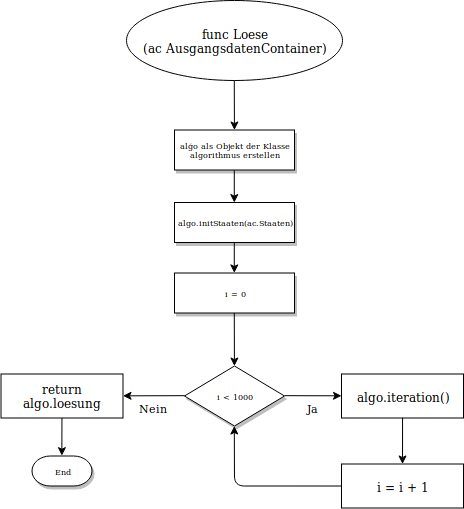
\includegraphics[width=0.9\textwidth,]{Loese.png}
    \caption[]{Funktion Loese}
\end{figure}

\FloatBarrier

\subsubsection{algorithmus}

Die Klasse algorithmus implementiert die Lösung des Problemes und speichert den aktuellen Stand der Lösung.
Zusätzlich hat sie ein Feld für Nachbarschaftsbeziehungen und eins für die aktuell in dieser Iteration berechneten Kräfte.
Die wichtigste Methode ist iteration(). Diese berechnet die nächste Iteration der Lösung.

\subsubsection{algorithmus.iteration()}
Die Methode Iteration ist der Kern des Algorithmus, hier werden die Kräfte berechnet und die Staaten verschoben.

\begin{figure}[h!]
    \centering
    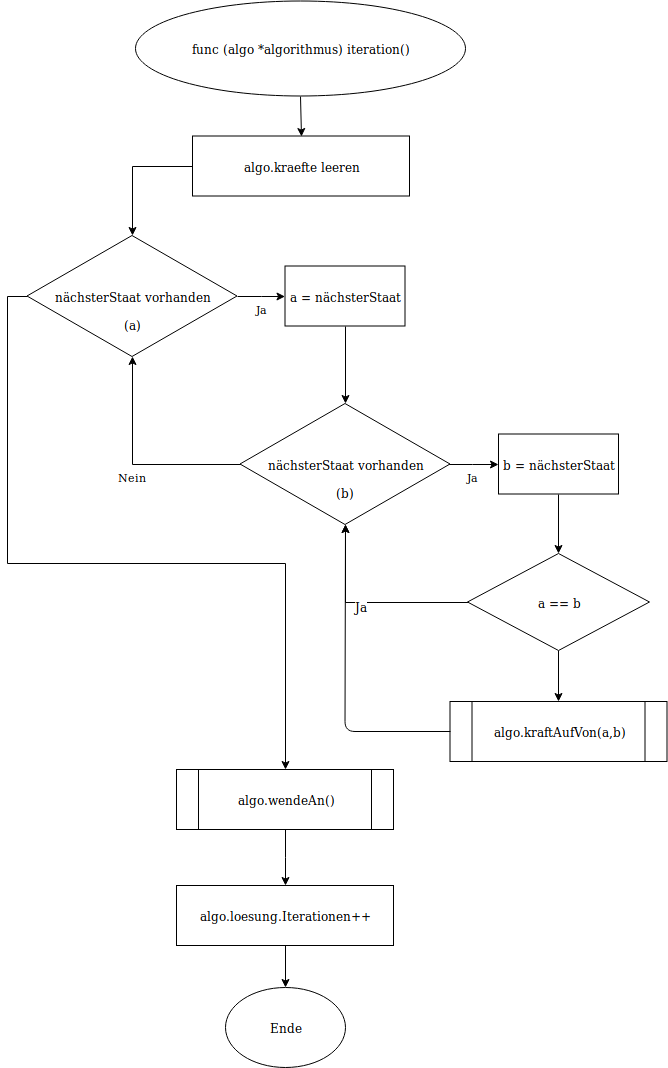
\includegraphics[width=0.55\textwidth,]{Iteration.png}
    \caption[]{Methode algorithmus.Iteration}
\end{figure}

\pagebreak

\subsubsection{algorithmus.kraftVonAuf()}
In der Methode kraftVonAuf wird die Kraft von Staat b auf Staat a berechnet.

\begin{figure}[h!]
    \centering
    \includegraphics[width=0.7\textwidth,]{kraftVonAuf.png}
    \caption[]{Methode algorithmus.kraftVonAuf}
\end{figure}

\FloatBarrier

\subsubsection{algorithmus.wendeAn()}

Die Methode wendeAn() wendet die berechneten Kräfte auf die Staaten an.

\begin{figure}[h!]
    \centering
    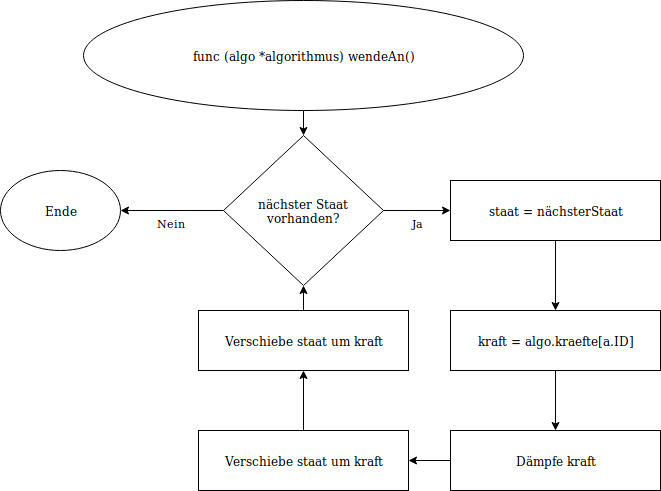
\includegraphics[width=0.8\textwidth,]{wendeAn.png}
    \caption[]{Methode algorithmus.wendeAn}
\end{figure}

\pagebreak

\subsection{Ausgabe}

Das Package ausgabe enthält die nötigen Funktionen um die Lösung für gnuplot aufzubereiten und in eine Ausgabedatei zu schreiben.

\subsubsection{GNUPlotToFile()}

Die Funktion GNUPlotToFile schreibt die Ausgabedatei in dem an gnuplot ausgerichtetetn Format.
Sie ruft dabei die Helferfunktion findExtrema auf um sicherzustellen das die xRange gleich groß wie die yRange ist.
Falls es einen Fehler beim erstellen der Datei gibt wird dieser zurückgegeben.

\subsubsection{findExtrema()}

findExtrema ist eine Helferfunktion um sicherzustellen das die xRange gleich groß wie die yRange ist und alle Staaten vollständig im Bild enthalten sind.
Dafür findet sie erst das kleinste Rechteck um alle Staaten herum und verlängert dann die kürzere Seite des Rechtecks gleichmäßig auf beiden Seiten um ein Quadrat zu erschaffen.

\begin{figure}[htb]
    \centering
    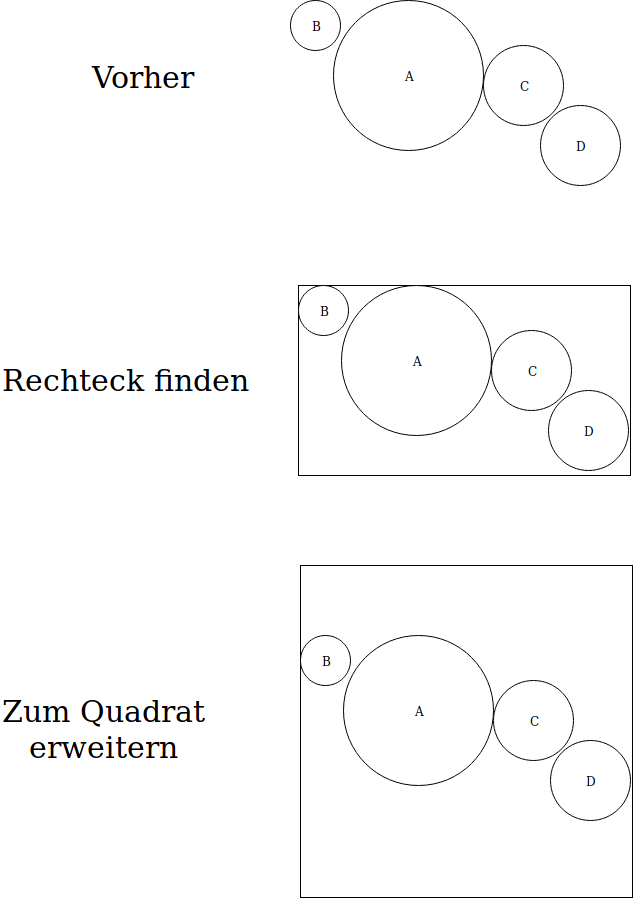
\includegraphics[width=0.4\textwidth,]{findExtrema.png}
    \caption[]{Funktion findExtrema}
\end{figure}
